\begin{tutorial}{Калькулятор пиццы}

Для решения задачи нужно набрать максимальное количество пицц одного размера и, 
возможно, по одной пицце других размеров.

Алгоритм должен выбрать в цикле максимизируемую пиццу, а затем
вычислить стоимость 4 вариантов для двух пицц других размеров:

\begin{center}
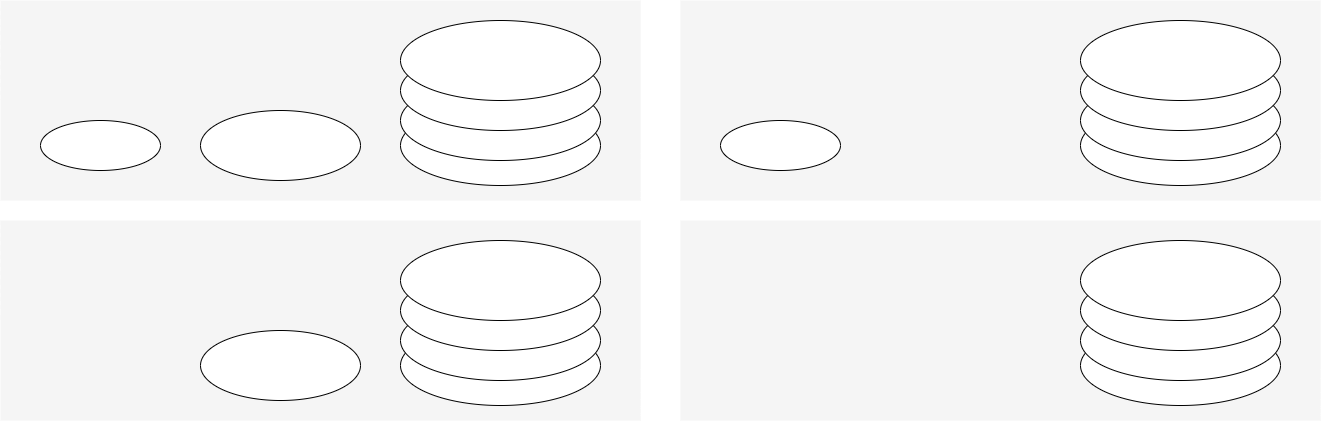
\includegraphics[scale=0.3]{pizza.png}
\end{center}

Вычислив стоимость этих 12 вариантов, нужно вывести наименьшую из них.


\end{tutorial}
